\section{The Structure Aspect}

After we have mined the structure of the language out of the grammar file, we can finally start working with MPS.
We need to translate our tree structure into the terms of MPS.
That means creating concepts inside the structure aspect and linking them together appropriately.
\\

We will describe several different attempts (sections \ref{chap:straightforward_approach} and \ref{chap:shortcut_approach}) the author has tried out and show some problems these attempts introduced.
We consider it a better approach than just simple description of the final solution because it might prevent others from falling into similar pitfalls such as we discovered ourselves.


\subsection{Concept Types}

Before we start describing how we decided to import our tree structure into MPS, we should remind in more detail which means of expression are available to us.
As stated before, concepts are building blocks of all MPS languages and they can be treated similarly as Java classes.
They can:

\begin{itemize}
	\item extend a parent concept
	\item inherit any number of interfaces (interface concepts)
	\item have properties (similar to class fields) with a given data type --- either a primitive type such as string or integer, or a constraint data type --- a string whose value is restricted by a regular expression
	\item have children concepts (defined as a concept or an interface concept)
	\item hold references to other nodes (e.g. function call statement would know reference to the function definition)
	\item have an \textit{alias} and a \textit{description} field for their better identification in auto-completion menus
\end{itemize}

\subsection{Common Ground}
\label{chap:common_ground}

Some of the import steps are common for both approaches (\ref{chap:straightforward_approach}, \ref{chap:shortcut_approach}).
\\

Firstly, we have noticed, that whenever there is a string literal inside a parser rule's alternative (think of the \textbf{for} keyword from a Java loop), it will appear only in that rule's projectional editor.
There is no need for it to have any function as it is set in stone as an unchangeable part of that alternative's appearance.
It might serve its purpose when describing or naming this alternative inside an auto-complete menu, but we will get to that part below.
\\

Secondly, we can take the flattened lexer rules, that contain the regular expression, we have built by gluing its parts together in the parsing stage.
For each one of these, we create a constraint data type concept, which is exactly what we need.
We will be able to later create properties of concepts and set their data type as this constraint data type concept, effectively restricting their value using given regular expression.
\\

Last, we take all literals found in the alternative and glue them together to one string, which we will use as the alias of the concept.
We will use the name of the parser rule, this alternative belongs to, as the description text for the concept.
\\

To illustrate what a concept for a sample alternative looks like, consider the element concept that represents the full XML tag with content:

\begin{antlr}
	\parserrule{element}      :   \literal{<} \lexerrule{Name} \parserrule{attribute}* \literal{>} \parserrule{content}* \literal{</} \lexerrule{Name} \literal{>}
             \textcolor{gray}{|   \ap<\ap Name attribute* \ap/>\ap}
             \textcolor{gray}{;}
\end{antlr}

Because we are creating a new concept for each alternative of the rule, we will be numbering them correspondingly.
The concept, that will represent the first alternative of the \parserrule{element} rule, will therefore be named \concept{Element{\_}1}
(we will mark concepts \concept{green} and interfaces \interface{purple}).

\begin{itemize}
	\item Since there are two references to the \lexerrule{Name} lexer rule inside the first alternative of the \parserrule{element} rule, the \concept{Element{\_}1} concept will contain two properties, whose value will be restricted using the regular expression representing the \lexerrule{Name} rule.
	We can achieve this using the \textit{Constraint data type concept}, which we create for each lexer rule.

	\item Literals are skipped (as explained above using the \textbf{for} keyword).

	\item Parser rules references (\parserrule{attribute} and \parserrule{content}) will be explained further down the road as they are the part where approaches differ.
\end{itemize}

Result of this first step can be seen in Figure \ref{fig:element_concept_common}.

\begin{figure}[h]
	\centering
	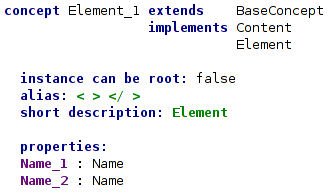
\includegraphics[scale=0.75]{./img/element_concept_common.png}
	\caption{Resulting Element{\_}1 concept}
	\label{fig:element_concept_common}
\end{figure}

Next, we are going to describe two different approaches --- the straightforward approach (section \ref{chap:straightforward_approach}) and the shortcut approach (section \ref{chap:shortcut_approach}).
The difference between these two lies in the way we create children fields for parser rules and in the way we are going to link them together using interface concepts.
Final solution will be described in section \ref{chap:structure_solution}.

\newpage

\subsection{The Straightforward Approach}
\label{chap:straightforward_approach}

The first attempt was quite straightforward and a little bit explorative, in the way that the author had to discover the MPS API that allows programmatical language generation.
Because MPS is still in development, the API isn't that well documented and some features had to be discovered through trial and error or through examination of the PE4MPS project (Section~\ref{chap:pe4mps}), which served great aid here.

\subsubsection{The Algorithm}
\label{chap:straight_algorithm}
The main idea behind the first attempt comes from the realization that when a parser rules breaks into more alternatives, we need to create a concept for each alternative.
Then we have to somehow mark them as belonging to that parser rule.
Consider the \parserrule{content} rule from our SimpleXML language:

\begin{antlr}
	\parserrule{content}    :   \lexerrule{TEXT}
           |   \parserrule{element}
           |   \parserrule{comment}
           |   \lexerrule{CDATA}
           ;
\end{antlr}

We will need to have 4 concepts that could appear anywhere the \parserrule{content} rule is referenced.
That is why we decided that for each rule with more than one alternative, we will create an interface concept.
Then for each alternative of this rule, we will create a concept that will implement this interface.
So for our \parserrule{content} example, we will get following setup:

\begin{antlr}
	\interface{IContent}   :   \concept{Content{\_}1}
           |   \concept{Content{\_}2}
           |   \concept{Content{\_}3}
           |   \concept{Content{\_}4}
\end{antlr}

Names of these concepts are derived from the name of the rule, numbers are added to alternatives correspondingly.
For rules with a single alternative, no interface is needed.
For rules that contain in-line block rules (Section~\ref{chap:subrules}), we have already created artificial parser rules in our tree representation during the parser phase (Section~\ref{chap:parsing_the_grammar}), which means we do not have to worry about them now.
\\

Now we will describe, how we linked parser rules together.
Consider the \parserrule{element} rule that is referencing the \parserrule{content} rule:

\begin{antlr}
	\parserrule{element}    :   \literal{<} \lexerrule{Name} \parserrule{attribute}* \literal{>} \parserrule{content}* \literal{</} \lexerrule{Name} \literal{>}
           |   \literal{<} \lexerrule{Name} \parserrule{attribute}* \literal{/>}
           ;
\end{antlr}

Following the algorithm mentioned above, there is one \interface{IElement} interface and two \concept{Element{\_}1}, \concept{Element{\_}2} concepts created.
For each referenced parser rule inside a concept, we create a child link and point it to the right interface.
In our example, for concept \concept{Element{\_}1}, there would be two child links pointing to \interface{IAttribute} and \interface{IContent}.
In Figure~\ref{fig:element_concept_full}, you can see the full \concept{Element{\_}1} concept.

\begin{figure}[h]
	\centering
	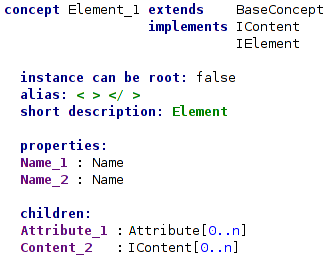
\includegraphics[scale=0.75]{./img/element_concept_full.png}
	\caption{Element{\_}1 concept's structure aspect}
	\label{fig:element_concept_full}
\end{figure}

Naming convention of child links also contains numbers, because names have to be unique.

\subsubsection{The Layer Problem}
\label{chap:layer_problem}

The algorithm mentioned above will leave us with an MPS language that follows given structure correctly and could be used to represent code in that language inside MPS correctly. Editing the code will not be possible yet, as there is no editor aspect defined so far.
There is one problem, however, concerning usability of such language.
We will demonstrate this problem on the SimpleXML language, using \parserrule{element} and \parserrule{content} rules:

\begin{antlr}
	\parserrule{content}    :   \lexerrule{TEXT}
           |   \parserrule{element}
           |   \parserrule{comment}
           |   \lexerrule{CDATA}
           ;

	\parserrule{element}    :   \literal{<} \lexerrule{Name} \parserrule{attribute}* \literal{>} \parserrule{content}* \literal{</} \lexerrule{Name} \literal{>}
           |   \literal{<} \lexerrule{Name} \parserrule{attribute}* \literal{/>}
           ;
\end{antlr}

When we would be editing code in this language, the MPS auto-complete would give us aid when filling out all properties and children of inserted concepts.
Imagine there is a freshly inserted \concept{Element{\_}1} concept (a concept representing the full XML element as is stated in the first alternative of the \parserrule{element} parser rule).
This setup can be seen in the left part of Figure~\ref{fig:layer_problem}.
Now, we would like to insert some content inside.
Let's say we would like to insert a nested XML element inside.
We would place the cursor in the content placeholder and press Ctrl+Space to view the auto-completion options.
\\

Following the algorithm mentioned above, we have created a child link of the \concept{Element{\_}1} concept of type \interface{IContent}.
There exist 4 concepts that implement the \interface{IContent} interface as per each alternative of the rule.
MPS evaluates this and gives us 4 options inside the auto-complete.
This auto-complete is captured in Figure~\ref{fig:layer_problem}.

\begin{figure}[h]
	\centering
	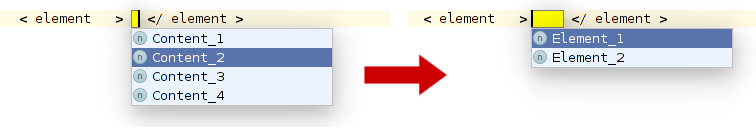
\includegraphics[width=\textwidth]{./img/layer_problem.png}
	\caption{Layer problem in auto-completion}
	\label{fig:layer_problem}
\end{figure}

In order to correctly insert another nested element inside, we would have to first insert a \concept{Content{\_}2} concept inside \concept{Element{\_}1} that has an \interface{IElement} child inside (and nothing else).
Then, as a second step, we would call for the auto-complete again and insert either \concept{Element{\_}1} or \concept{Element{\_}2} inside \concept{Content{\_}2}.
This mean that we have to go through two steps and in the first one either guess correctly (or remember the grammar rule's alternative order), to know, which item of the auto-complete we should go with.
\\

And the problem goes both ways --- if we decide to replace the nested \concept{Element{\_}1} with, let's say, an XML comment (a \concept{Comment} concept), we need to delete both intermediary layers before we get back to the original \concept{Content{\_}X} crossroads.
Meanwhile, the user cannot really see, what is happening, since the intermediary level has no appearance or indicator.
This leads to confusion on user's part.
\\

We tried to ease this situation up by creating aliases for concepts derived from their content (names such as “Element content” or “CDATA content” instead of Content{\_}N), but the problem goes beyond this.
Take into consideration that the SimpleXML grammar is a very simple one.
More sophisticated languages may have more than two intermediary layers and writing code would consist of clicking through a large number of auto-completes like shown in the example above.
There is also nothing preventing authors of grammars from naming these helper layers in a completely unrelated manner, which would make user's orientation even harder.
After all, these layers come into existence when the grammar is being written, so that it is more readable for humans and maybe better maintainable by the author.
It has nothing to do with making the AST simple for the ANTLR parser.
ANTLR is very capable and handles this probably very well in any form.
\\

Furthermore, using in-line subrule blocks makes this even a bigger problem as the block rule's names are auto-generated by our parser and differ only by numbers, even though the alias assigning process improves the situation by a bit.
But from the point of view of the grammar's author, it is an invisible layer of rules nested inside.



\subsection{The shortcut approach}
\label{chap:shortcut_approach}

After the problem with layers crossed our path in the first attempt, we took a step back and tried to reevaluate our approach.
The second attempt is based on looking at elements of alternatives (parser rule references) and asking: "which concepts could be inserted in this place?".
Consider again the \parserrule{content} rule and its child rules:

\begin{antlr}
	\parserrule{content}    :   \lexerrule{TEXT}
           |   \parserrule{element}
           |   \parserrule{comment}
           |   \lexerrule{CDATA}
           ;

	\parserrule{element}    :   \literal{<} \lexerrule{Name} \parserrule{attribute}* \literal{>} \parserrule{content}* \literal{</} \lexerrule{Name} \literal{>}
           |   \literal{<} \lexerrule{Name} \parserrule{attribute}* \literal{/>}
           ;

	\parserrule{comment}    :   \literal{<!--} \lexerrule{TEXT} \literal{-->} ;
\end{antlr}

We started building on top of the algorithm mentioned in \ref{chap:straight_algorithm}.
This leaves us again with a concept for each alternative and an interface for parser rules containing more alternatives.
We can see that the content rule can ultimately expand into following concepts:

\begin{itemize}
	\item \textbf{Content{\_}1} (TEXT)
	\item Content{\_}2 $\rightarrow$ \textbf{Element{\_}1}
	\item Content{\_}2 $\rightarrow$ \textbf{Element{\_}2}
	\item Content{\_}3 $\rightarrow$ \textbf{Comment}
	\item \textbf{Content{\_}4} (CDATA)
\end{itemize}

The layer problem (\ref{chap:layer_problem}) dwells in the need of inserting the \concept{Content{\_}2} concept before being able to insert one of the \concept{Element{\_}1} or \concept{Element{\_}2} concepts.
We would like to avoid that and offer directly the concepts that are at the end of the chain (in bold).
These are concepts we would like to see in the auto-completion menu.
They cannot transparently break into more rules and for the sake of text we will call them \textbf{end concepts}, or when talking about the grammar rule tree \textbf{end rules}. 
\\

We will describe an algorithm, that will find all end rules for a given parser rule, and later utilize it.

\subsubsection{The algorithm}
To find end rules for each parser rule, we can recursively scan through the parser tree, that we have built before. For each parser rule, we will try to find paths leading to some end rule through its alternatives:

\begin{itemize}
	\item Whenever we find an alternative, that contains only one element, and this element is a reference to another parser rule, we have found an intermediary level that can be transparently hidden from the user of the language. 
	We will continue recursively processing alternatives of this “level” rule (we are not at the end of the chain yet).

	\item Otherwise, we have found an end rule (recursion stops here).
\end{itemize}

We have expressed this algorithm using a pseudo-code:

\label{chap:shortcut_algorithm}
\begin{antlr}
	FindPathsToEndNodes(\parserrule{R}):
	1)  Define \parserrule{L} as an empty list of list of nodes
	2)  Return FindPathsToEndNodes(\parserrule{R}, \parserrule{L})
	
	FindPathsToEndNodes(\parserrule{R}, \parserrule{L}):
	3)  Define \parserrule{Q} as list of list of nodes
	4)  For each alternative \parserrule{A} of rule \parserrule{R}:
	5)      \parserrule{L1} = Clone(\parserrule{L})
	6)      If \parserrule{A} is a parser rule with only one element \parserrule{E}:
	7)          Let \parserrule{I} be interface/concept representing rule \parserrule{E}
	8)          \parserrule{L1}.Add(\parserrule{I})
	9)          \parserrule{P} = FindPathsToEndNodes(\parserrule{E}, \parserrule{L1})
	10)          \parserrule{Q} = Merge(\parserrule{Q}, \parserrule{P})
	11)      Else
	12)          \parserrule{L1}.Add(\parserrule{R})
	13)          Let \parserrule{P} be concept representing \parserrule{A}
	14)          \parserrule{L1}.Add(\parserrule{P})
	15)          \parserrule{Q}.Add(\parserrule{L1})
	16)  Return \parserrule{Q}
\end{antlr}

By appending the rule that is leading to current element (line 12) and then appending that alternative's element itself (line 14), we will get a path that contains the full path and the target end rule as the last element of the chain.
The result of this algorithm, for example for the \parserrule{content} rule, equals the listing of the five paths mentioned in the beginning of this chapter.
\\

We can do this for all parser rules and for each rule we will get a list of paths that lead from that particular rule to an end node. 
We will call these paths \textbf{shortcuts}, as they can provide a shortcut from the rule to the end of chain. 
Now that we have these, we will talk about several ways, how to use them to make our language better.

\subsubsection{Smart auto-completion}
The first attempt on how to use shortcuts (result of the algorithm in \ref{chap:shortcut_algorithm}) was built on top of the previous approach. 
There were no structural changes when it came to interfaces or linking concepts together.
We imported everything just the same and then added some more functionality.
\\

We were trying to solve the most obvious problem in front of us --- the auto-completion. 
We would like to improve it, so that it offers us only end concepts.
Luckily for us, MPS gives us the ability to create custom auto-complete menus and use those instead of the built-in one.
This means, that we are going to be able to construct our own menu containing only end nodes.
Unfortunately, it requires us to implement some non-trivial mechanisms.

\paragraph{Defining the auto-complete}

The auto-complete menu is bound to a cell of the projectional editor containing a reference to one of the children of a concept.
Let's say we are again talking about the concept that represents the element rule's first alternative.
As described above earlier in the process (\ref{fig:element_concept_full}), we created:

\begin{itemize}
	\item An interface \interface{IContent} representing four different alternatives that the content rule can break into

	\item A child of the \concept{Element{\_}1} concept, that references the \interface{IContent} rule
\end{itemize}

Somewhere in the editor aspect of the \concept{Element{\_}1} concept, there will be a cell referencing the concept interface \interface{IContent}. 
The cell, together with the auto-complete property can be seen in figure \ref{fig:autocomplete_cell}.

\begin{figure}[h]
	\centering
	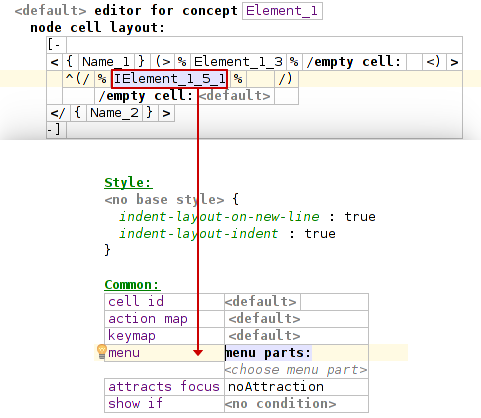
\includegraphics[width=\textwidth]{./img/autocomplete_cell.png}
	\caption{Auto-complete property \textbf{[TODO: edit image]}}
	\label{fig:autocomplete_cell}
\end{figure}

We would like to create an auto-complete for this cell, that would contain following options (end concepts):

\begin{itemize}
	\item Content{\_}1
	\item Element{\_}1
	\item Element{\_}2
	\item Comment
	\item Content{\_}4
\end{itemize}

Because we are inside MPS everything is a concept node.
In order to create an auto-complete menu, we need to create some BaseLanguage node and put it inside some AST (referencing the menu).
More precisely, we will create an instance a concept called \texttt{CellMenuPart{\_}ReplaceChild{\_}CustomActionConcept}, contained in one of many MPS's core languages.
\\

For this concept we will define a number of auto-complete options, one for each end concept, that we want to offer in the menu.
Every option has a \textbf{textual description}, \textbf{matching text} (so that we can filter through them) and most importantly a \textbf{creator method}.
If user selects that particular option, this method will be called with some contextual information in parameters and it is expected to return an instance of some concept that implements the \interface{IContent} interface.
\\

The complicated part of the process comes now, as we would like to dynamically generate the creator method.
We need to create BaseLanguage statements, that will instantiate the end concept and return it.
There is one small problem though.
Let's say the user selected the second option and decided to insert another \concept{Element{\_}1} inside.
The problem is, that \concept{Element{\_}1} doesn't implement the \interface{IContent} interface.
It only implements the \interface{IElement} interface as per the algorithm of the straightforward approach (\ref{chap:straight_algorithm}).
The shortcut, that leads to this end concept leads through the \concept{Content{\_}2} concept, that has an Element child.
This means, that we have to follow the whole path and chain individual nodes, beginning with the \concept{Content{\_}2} concept.
For this particular case it would mean to:

\begin{itemize}
	\item Create an \concept{Element{\_}1} concept and store it in a variable.

	\item Create a \concept{Content{\_}2} concept and store it in a variable.

	\item Assign the \concept{Element{\_}1} node to the right child of the \concept{Content{\_}2} node.

	\item Return \concept{Content{\_}2} node.
\end{itemize}

As we said earlier in section \ref{chap:generating_code_inside_mps}, generating BaseLanguage code is a bit more complicated because we need to either use quotation or create a large number of AST nodes. Using quotation in this case was sometimes impossible as everything is very dynamic. The finished option concept is shown in figure \ref{fig:autocomplete_action}.

\begin{figure}[h]
	\centering
	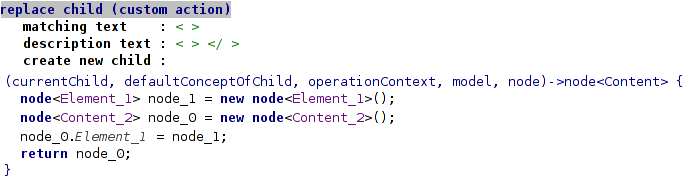
\includegraphics[width=\textwidth]{./img/autocomplete_action.png}
	\caption{Auto-complete action code (Element{\_}1 concept)}
	\label{fig:autocomplete_action}
\end{figure}

For the description text, we used concept's alias. We talk about creating aliases in chapter [TODO: alias chapter reference].
For matching text we used the shortest unique prefix of alias among all other options' aliases in given auto-complete menu.
The algorithm for searching shortest unique prefixes in a set of strings is not important from our thesis' point of view, so we decided to not go into further detail.

\paragraph{The layer problem again [TODO]}

After we implemented the auto-complete menu, coding in the imported language started to be very reasonable and comfortable since we eradicated intermediate layers. Or did we? When producing code, the language really does what one would expect, however when user starts deleting things, the layer problem occurs once more.
\\

What happens here is that when we select the auto-complete option, several layers of concept might get created and inserted into the cell. Imagine we just inserted the \concept{Element{\_}1} node. According to the creator method, this new node is wrapped inside of the \concept{Content{\_}2} node. Now let's say user changed his mind and wants to replace this XML element with a comment. He would press backspace, the XML element would disappear as expected. Then user would invoke the auto-complete menu again and expect again to have all five options at hand. What happened instead is that the \concept{Element{\_}1} node got deleted, but the wrapping \concept{Content{\_}2} one remained. The \concept{Content{\_}2} concept has only one child of type Element and that is why user only sees \concept{Element{\_}1} and \concept{Element{\_}2} as options in the auto-complete.

\paragraph {The deletion context}

Solution to this resurrected layer problem lies in controlling the deletion event. Once again, MPS' authors have equipped us with tools for doing this. We are able to specify our own handler for the deletion event for any cell of the projectional editor. But what will it look like?
\\

When deleting a node, we would like to remove the shortcut, the whole path, and effectively reversing the effect of the creator method. We decided that it will be the easiest to store the length of the path that is leading to certain node with the node. So when we are creating the node path in the creator method, we tell each node how deep or far on the path it is. In order to do this, we created a \concept{BaseConcept}, a parent abstract concept from which we will inherit all other concepts. This abstract concept will define a special integer property that will hold our information and effectively making all other concepts inherit it too. We called this property \textit{{\_}{\_}DeleteContext} and enhanced the creator method as shown in figure \ref{fig:autocomplete_action_delete_context}.

\begin{figure}[h]
	\centering
	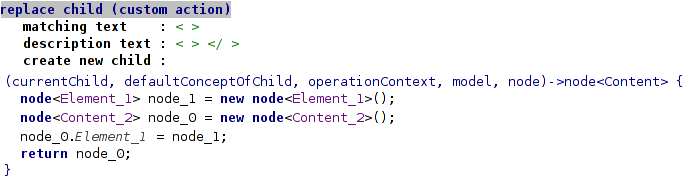
\includegraphics[width=\textwidth]{./img/autocomplete_action_delete_context.png}
	\caption{Auto-complete action extended with deletion context}
	\label{fig:autocomplete_action_delete_context}
\end{figure}

The last thing remaining is creating the backspace action. Apart from some problems with referencing the \textit{{\_}{\_}DeleteContext} property, which must be reached through the abstract \concept{BaseConcept} type, it is quite straightforward to generate a BaseLanguage code like shown below (figure \ref{fig:backspace_action}).

\begin{figure}[h]
	\centering
	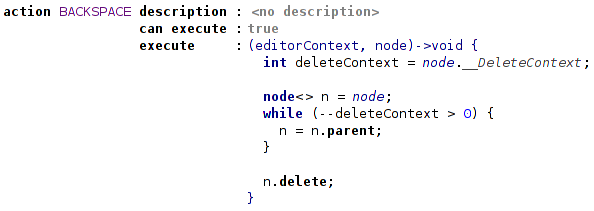
\includegraphics[width=\textwidth]{./img/backspace_action.png}
	\caption{Backspace action implementation}
	\label{fig:backspace_action}
\end{figure}

We must not forget to pin this handler to every cell that we pin the auto-complete to. After we had done this, the layer problem has finally been eradicated. The language became a bit more usable once more.

\subsubsection{Smart interfaces}

After we have implemented the smart autocomplete, we realized that there might be another way to accomplish almost the same result. It would mean changing the first step concerning concept interfaces creation.
\\

The main idea behind this is the realization that if for each concept interface there exists a finite set of end concepts, we could just create a special interface and let all these and only these end concepts implement it. It is important that other non-end concepts that are in the shortcut will not implement it, because that would put us right back where we started with the straightforward approach \ref{chap:straightforward_approach} and the layer problem \ref{chap:layer_problem}. To give an example regarding our content rule, we would create an \interface{IContent} interface concept and only following concepts would implement it:

\begin{itemize}
	\setlength\itemsep{0pt}
	\item Content{\_}1
	\item Element{\_}1
	\item Element{\_}2
	\item Comment
	\item Content{\_}4
\end{itemize}

Concepts would of course implement as many interfaces as many shortcuts lead to them. The difference is that the intermediary layers will not, preventing the layering.
\\

We still need to find end concepts for each rule, so we will keep the same algorithm for finding shortcuts as before. We, however, do not need to implement our own auto-completion (and subsequently with it no deletion handlers), because the built in default auto-completion will start to behave exactly the same way our smart auto-completion did.

\paragraph{Cardinality restriction}

So far it looks like the last approach is superior to the auto-completion one. It avoids complicated code generation and even resulting MPS languages are more simple, perhaps better performant as they are not bloated with auto-completion code. There is one small drawback though, that makes this solution suboptimal.
\\

To remind the reader --- the cardinality of an element is telling us, how many of each specific child rules can occur inside an alternative. Inside the grammar this was expressed using quantification operators (\textbf{*},\textbf{+} and \textbf{?}). The problem that appears here can be shown using these example rules:

\begin{antlr}
\parserrule{content}      :   \parserrule{element}+
             |   \parserrule{comment}*
             |   \lexerrule{CDATA}?
             ;
\end{antlr}

Notice, how we changed the cardinality of elements inside the \parserrule{content} rule. This small change will prevent us from creating a shortcut leading through this rule. We are trying to say that shortcuts that can be used for the smart interfaces approach can only lead through rules, that have cardinality [1..1] (so through an alternative with a single child element, that is a reference to a parser rule AND has this cardinality). Speaking in terms of the shortcut algorithm \ref{chap:shortcut_algorithm}, we would alter line number 6 and add this restriction to the condition.
\\

This restriction is caused by the fact that we would be unable to control children cardinality. Imagine that some alternative of some other rule contains reference to this altered \parserrule{content} rule (regardless of its quantitative operator). That means that we need to create a child holding the \interface{IContent} and setting this cardinality. But each alternative of the altered content rule requires different number of children to be inserted. Since there are no intermediary levels of nodes that could influence this, the end concept node that would be inserted in that child would inherit the cardinality of the child regardless of what the shortcut path looks like.
\\

A small example might demonstrate this better. We have an \interface{IContent} [1..1] child. If we disregarded the cardinality restriction, we could ultimately put there \concept{Element{\_}1} end concept node. But the content rule says, there can be [1..n] elements. We are still bound to insert only one though.


\subsection{Our Solution}
\label{chap:structure_solution}

In the end, we have decided to go with the shortcut approach using smart interfaces.
As we have stated above, it has several advantages, concerning the solution complexity, compared to the smart auto-completion.
It only has one disadvantage regarding the cardinality restriction, described in \ref{chap:cardinality_restriction}.
We have analyzed several ANTLR grammars (such as the JavaScript~\cite{javascript}) and we haven't found a single intermediate rule, that would be suffering from this restriction.
It is quite understandable if you think about how grammars are written.
Usually, you create the basic structure (i.e. different kinds of statements) in the simplest way possible and put the quantitative operator rather to an alternative that is referencing the structure.
\\

Based on these observations and some grammar analysis, we concluded that advantages prevail and used the last mentioned approach.

\subsection{The Structure Aspect and Other ANTLRv4 Features}
\label{chap:antlr_features}

The ANTLR grammar notation offers more features than just rule definition.
We haven't mentioned these earlier because we were focusing solely on the structure of the language.
We will mention some features and explain why we have ignored them and why they don't matter to us.
We will not spend a lot of time on describing details of these as they are well documented in the official ANTLR reference~\cite{ANTLR4reference}.

\subsubsection{Modes}

For example, just like any other parser/lexer, ANTLR gives us the possibility to switch the parsing context.
We are able to create various user-specified modes and then enter these modes when certain rules/tokens are encountered.
For each mode, we can define a different set of rules/tokens that can only be applied when the parser is in that particular mode.
The syntax is following:

\begin{antlr}
	\textcolor{gray}{// Enter mode when tag opened}
	\lexerrule{OPEN}        :   \literal{<}       -> pushMode(INSIDE) ;

	mode INSIDE;
	\textcolor{gray}{// Special rules bound to specific mode}
	\lexerrule{S}           :   \regex{[ {\textbackslash}t{\textbackslash}r{\textbackslash}n]} -> skip ;

	\textcolor{gray}{// Leave the mode when tag closed}
	\lexerrule{CLOSE}       :   \literal{>}       -> popMode ;
	\lexerrule{SLASH{\_}CLOSE} :   \literal{/>}      -> popMode ;
\end{antlr}

We didn't pay any extra attention to modes while dealing with the structural aspect because they don't really influence contents of individual concepts.
It is even possible to define concepts that control mode switching and then not including them inside any parser rule.
They still get recognized by the lexer and mode is changed.
\\

The reason that this goes beyond our interest here is partially caused by the fact, that modes are used on runtime when we are parsing actual code, whereas language structure is more of a static matter.
The only time we care about modes is when generating the TextGen aspect, and we will get back to it later in Chapter \ref{chap:textgen}.

\subsubsection{Actions, Attributes and Semantic Predicates}

Actions allow us to append code to rules and this code is then executed every time the parser applies this rule.
The code is written in the target language that you are creating the parser for.
It is then copied as a string and inserted into the method that is bound to parsing this rule.
Again, this is of a little interest to us.
Usually, this is used when creating some specific parsers for some particular scenario.
We, however, are expecting to parse general purpose languages that contain actions just rarely.
And even when they did, we cannot be sure what language will it be in and how to use it.
\\

Attributes allow us to extend some basic predefined set of properties of each rule.
We can store some arbitrary information there and later access it for example inside actions using special syntax.
From exactly the same reasons as with actions, attributes are of no interest to us.
\\

Semantic predicates tell the parser on runtime, which rules can be applied depending on specified constraints.
This is also a runtime matter.
